% Options for packages loaded elsewhere
\PassOptionsToPackage{unicode}{hyperref}
\PassOptionsToPackage{hyphens}{url}
%
\documentclass[
]{article}
\usepackage{amsmath,amssymb}
\usepackage{iftex}
\ifPDFTeX
  \usepackage[T1]{fontenc}
  \usepackage[utf8]{inputenc}
  \usepackage{textcomp} % provide euro and other symbols
\else % if luatex or xetex
  \usepackage{unicode-math} % this also loads fontspec
  \defaultfontfeatures{Scale=MatchLowercase}
  \defaultfontfeatures[\rmfamily]{Ligatures=TeX,Scale=1}
\fi
\usepackage{lmodern}
\ifPDFTeX\else
  % xetex/luatex font selection
\fi
% Use upquote if available, for straight quotes in verbatim environments
\IfFileExists{upquote.sty}{\usepackage{upquote}}{}
\IfFileExists{microtype.sty}{% use microtype if available
  \usepackage[]{microtype}
  \UseMicrotypeSet[protrusion]{basicmath} % disable protrusion for tt fonts
}{}
\makeatletter
\@ifundefined{KOMAClassName}{% if non-KOMA class
  \IfFileExists{parskip.sty}{%
    \usepackage{parskip}
  }{% else
    \setlength{\parindent}{0pt}
    \setlength{\parskip}{6pt plus 2pt minus 1pt}}
}{% if KOMA class
  \KOMAoptions{parskip=half}}
\makeatother
\usepackage{xcolor}
\usepackage[margin=1in]{geometry}
\usepackage{color}
\usepackage{fancyvrb}
\newcommand{\VerbBar}{|}
\newcommand{\VERB}{\Verb[commandchars=\\\{\}]}
\DefineVerbatimEnvironment{Highlighting}{Verbatim}{commandchars=\\\{\}}
% Add ',fontsize=\small' for more characters per line
\usepackage{framed}
\definecolor{shadecolor}{RGB}{248,248,248}
\newenvironment{Shaded}{\begin{snugshade}}{\end{snugshade}}
\newcommand{\AlertTok}[1]{\textcolor[rgb]{0.94,0.16,0.16}{#1}}
\newcommand{\AnnotationTok}[1]{\textcolor[rgb]{0.56,0.35,0.01}{\textbf{\textit{#1}}}}
\newcommand{\AttributeTok}[1]{\textcolor[rgb]{0.13,0.29,0.53}{#1}}
\newcommand{\BaseNTok}[1]{\textcolor[rgb]{0.00,0.00,0.81}{#1}}
\newcommand{\BuiltInTok}[1]{#1}
\newcommand{\CharTok}[1]{\textcolor[rgb]{0.31,0.60,0.02}{#1}}
\newcommand{\CommentTok}[1]{\textcolor[rgb]{0.56,0.35,0.01}{\textit{#1}}}
\newcommand{\CommentVarTok}[1]{\textcolor[rgb]{0.56,0.35,0.01}{\textbf{\textit{#1}}}}
\newcommand{\ConstantTok}[1]{\textcolor[rgb]{0.56,0.35,0.01}{#1}}
\newcommand{\ControlFlowTok}[1]{\textcolor[rgb]{0.13,0.29,0.53}{\textbf{#1}}}
\newcommand{\DataTypeTok}[1]{\textcolor[rgb]{0.13,0.29,0.53}{#1}}
\newcommand{\DecValTok}[1]{\textcolor[rgb]{0.00,0.00,0.81}{#1}}
\newcommand{\DocumentationTok}[1]{\textcolor[rgb]{0.56,0.35,0.01}{\textbf{\textit{#1}}}}
\newcommand{\ErrorTok}[1]{\textcolor[rgb]{0.64,0.00,0.00}{\textbf{#1}}}
\newcommand{\ExtensionTok}[1]{#1}
\newcommand{\FloatTok}[1]{\textcolor[rgb]{0.00,0.00,0.81}{#1}}
\newcommand{\FunctionTok}[1]{\textcolor[rgb]{0.13,0.29,0.53}{\textbf{#1}}}
\newcommand{\ImportTok}[1]{#1}
\newcommand{\InformationTok}[1]{\textcolor[rgb]{0.56,0.35,0.01}{\textbf{\textit{#1}}}}
\newcommand{\KeywordTok}[1]{\textcolor[rgb]{0.13,0.29,0.53}{\textbf{#1}}}
\newcommand{\NormalTok}[1]{#1}
\newcommand{\OperatorTok}[1]{\textcolor[rgb]{0.81,0.36,0.00}{\textbf{#1}}}
\newcommand{\OtherTok}[1]{\textcolor[rgb]{0.56,0.35,0.01}{#1}}
\newcommand{\PreprocessorTok}[1]{\textcolor[rgb]{0.56,0.35,0.01}{\textit{#1}}}
\newcommand{\RegionMarkerTok}[1]{#1}
\newcommand{\SpecialCharTok}[1]{\textcolor[rgb]{0.81,0.36,0.00}{\textbf{#1}}}
\newcommand{\SpecialStringTok}[1]{\textcolor[rgb]{0.31,0.60,0.02}{#1}}
\newcommand{\StringTok}[1]{\textcolor[rgb]{0.31,0.60,0.02}{#1}}
\newcommand{\VariableTok}[1]{\textcolor[rgb]{0.00,0.00,0.00}{#1}}
\newcommand{\VerbatimStringTok}[1]{\textcolor[rgb]{0.31,0.60,0.02}{#1}}
\newcommand{\WarningTok}[1]{\textcolor[rgb]{0.56,0.35,0.01}{\textbf{\textit{#1}}}}
\usepackage{graphicx}
\makeatletter
\def\maxwidth{\ifdim\Gin@nat@width>\linewidth\linewidth\else\Gin@nat@width\fi}
\def\maxheight{\ifdim\Gin@nat@height>\textheight\textheight\else\Gin@nat@height\fi}
\makeatother
% Scale images if necessary, so that they will not overflow the page
% margins by default, and it is still possible to overwrite the defaults
% using explicit options in \includegraphics[width, height, ...]{}
\setkeys{Gin}{width=\maxwidth,height=\maxheight,keepaspectratio}
% Set default figure placement to htbp
\makeatletter
\def\fps@figure{htbp}
\makeatother
\setlength{\emergencystretch}{3em} % prevent overfull lines
\providecommand{\tightlist}{%
  \setlength{\itemsep}{0pt}\setlength{\parskip}{0pt}}
\setcounter{secnumdepth}{-\maxdimen} % remove section numbering
\ifLuaTeX
  \usepackage{selnolig}  % disable illegal ligatures
\fi
\usepackage{bookmark}
\IfFileExists{xurl.sty}{\usepackage{xurl}}{} % add URL line breaks if available
\urlstyle{same}
\hypersetup{
  pdftitle={Social network analysis HW1: export-network},
  pdfauthor={Yijia Lin, Diego Paroli},
  hidelinks,
  pdfcreator={LaTeX via pandoc}}

\title{Social network analysis HW1: export-network}
\author{Yijia Lin, Diego Paroli}
\date{2025-04-23}

\begin{document}
\maketitle

\section{Libraries}\label{libraries}

\begin{Shaded}
\begin{Highlighting}[]
\FunctionTok{rm}\NormalTok{(}\AttributeTok{list =} \FunctionTok{ls}\NormalTok{())}
\FunctionTok{library}\NormalTok{(tidyverse)}
\FunctionTok{library}\NormalTok{(httr2)}
\FunctionTok{library}\NormalTok{(igraph)}
\FunctionTok{library}\NormalTok{(visNetwork)}
\FunctionTok{library}\NormalTok{(tidygraph)}
\FunctionTok{library}\NormalTok{(ggraph)}
\end{Highlighting}
\end{Shaded}

\section{Get the data}\label{get-the-data}

Data has been obtained following the procedure in the chunk below. The
code is commented to avoid repeating the download every time the notebok
is run.

\begin{Shaded}
\begin{Highlighting}[]
\CommentTok{\# zip\_data \textless{}{-} request("https://networks.skewed.de/net/product\_space/files/SITC.csv.zip") |\textgreater{}}
\CommentTok{\#   req\_perform()}
\CommentTok{\# }
\CommentTok{\# writeBin(resp\_body\_raw(zip\_data), "exports\_SITC.csv.zip")}
\CommentTok{\# }
\CommentTok{\# unzip("exports\_SITC.csv.zip", exdir = "network{-}data")}
\CommentTok{\# }
\CommentTok{\# file.remove("exports\_SITC.csv.zip", )}
\end{Highlighting}
\end{Shaded}

\begin{Shaded}
\begin{Highlighting}[]
\NormalTok{nodes }\OtherTok{\textless{}{-}} \FunctionTok{read\_csv}\NormalTok{(}\StringTok{"network{-}data/nodes.csv"}\NormalTok{)}
\NormalTok{links }\OtherTok{\textless{}{-}} \FunctionTok{read\_csv}\NormalTok{(}\StringTok{"network{-}data/edges.csv"}\NormalTok{)}
\end{Highlighting}
\end{Shaded}

\section{Description of the dataset}\label{description-of-the-dataset}

Our network represents economic products. Two products are connected if
two or more countries export both products in significant quantities
(above world average). The meaning of a link is that two products are
connected if the same countries ``specialize'' in making them, hence,
basically, products are connected if they require the same capabilities
to be made. Edges weights represent a similarity score (called
``proximity''). Data is based on UN Comtrade worldwide trade patterns
using the SITC (Standard International Trade Classification) for
classifying product categories.

Source: \href{https://www.michelecoscia.com/?page_id=223}{The Product
Space}.

\subsubsection{Properties:}\label{properties}

Weighted, Undirected

\subsubsection{Nodes and links}\label{nodes-and-links}

\begin{Shaded}
\begin{Highlighting}[]
\FunctionTok{head}\NormalTok{(nodes)}
\end{Highlighting}
\end{Shaded}

\begin{verbatim}
## # A tibble: 6 x 9
##   `# index`   pid community  size pos                  leamer name  color `_pos`
##       <dbl> <dbl>     <dbl> <dbl> <chr>                 <dbl> <chr> <chr> <chr> 
## 1         0  6932         0  48.8 array([4551.8996582~      8 WIRE~ "#9c~ array~
## 2         1  7362         0  65.2 array([ 216.8350982~      9 META~ "#40~ array~
## 3         2  7911         0  54.0 array([ 538.9149017~      9 RAIL~ "#40~ array~
## 4         3  8946         0  57.7 array([ 696.3942565~      7 NON-~ "#40~ array~
## 5         4  7264         0  73.3 array([  57.2840652~      9 PRIN~ "#40~ array~
## 6         5  2783         0  58.3 array([4662.2502441~      2 COMM~ "#ff~ array~
\end{verbatim}

\begin{Shaded}
\begin{Highlighting}[]
\FunctionTok{head}\NormalTok{(links)}
\end{Highlighting}
\end{Shaded}

\begin{verbatim}
## # A tibble: 6 x 4
##   `# source` target width color      
##        <dbl>  <dbl> <dbl> <chr>      
## 1          1    328  5.58 "#727272\n"
## 2          4    475  6.36 "#7b7b7b\n"
## 3          6     69  5.71 "#737373\n"
## 4          8     18  5.12 "#6c6c6c\n"
## 5          8      9  3.72 "#545454\n"
## 6         10    480  8.92 "#949494\n"
\end{verbatim}

Most of the columns in the \texttt{nodes} dataset will not be useful for
us. The column \texttt{\#\ index} is the one indicating the index of the
nodes and the column \texttt{name} is the one indicating their
corresponding name. In the \texttt{links} dataframe, the column
\texttt{\#\ source} and \texttt{target} indicate the 2 nodes forming a
link, while \texttt{width} is the weight of that link.

\subsubsection{Graph:}\label{graph}

\begin{Shaded}
\begin{Highlighting}[]
\NormalTok{graph }\OtherTok{\textless{}{-}} \FunctionTok{graph\_from\_data\_frame}\NormalTok{(links, }\AttributeTok{directed =} \ConstantTok{FALSE}\NormalTok{, }\AttributeTok{vertices =}\NormalTok{ nodes)}
\NormalTok{graph}
\end{Highlighting}
\end{Shaded}

\begin{verbatim}
## IGRAPH 0ef3264 UN-- 774 1779 -- 
## + attr: name (v/c), pid (v/n), community (v/n), size (v/n), pos (v/c),
## | leamer (v/n), color (v/c), _pos (v/c), width (e/n), color (e/c)
## + edges from 0ef3264 (vertex names):
## [1] METAL FORMING MACHINE TOOLS                    --CONVERTERS,LADLES,INGOT MOULDS AND CASTING MACH.  
## [2] PRINTING PRESSES                               --OTHER MACH.-TOOLS FOR WORKING METAL OR MET.CARBIDE
## [3] OTHER FOOD PROCESSING MACHINERY AND PARTS      --PARTS OF THE MACHINERY OF 744.2-                  
## [4] PRODUCER GAS AND WATER GAS GENERATORS AND PARTS--OTHER PUMPS FOR LIQUIDS & LIQUID ELEVATORS        
## [5] PRODUCER GAS AND WATER GAS GENERATORS AND PARTS--CINEMATOGRAPHIC CAMERAS,PROJECTORS,SOUND-REC,PAR  
## + ... omitted several edges
\end{verbatim}

\section{Questions}\label{questions}

\subsection{1. What is the number of nodes and
links?}\label{what-is-the-number-of-nodes-and-links}

\begin{Shaded}
\begin{Highlighting}[]
\FunctionTok{vcount}\NormalTok{(graph)}
\end{Highlighting}
\end{Shaded}

\begin{verbatim}
## [1] 774
\end{verbatim}

\begin{Shaded}
\begin{Highlighting}[]
\FunctionTok{ecount}\NormalTok{(graph)}
\end{Highlighting}
\end{Shaded}

\begin{verbatim}
## [1] 1779
\end{verbatim}

There are in total 774 nodes (i.e.~economic product) and 1779 links in
this network.

\begin{Shaded}
\begin{Highlighting}[]
\NormalTok{components }\OtherTok{\textless{}{-}} \FunctionTok{components}\NormalTok{(graph)}
\FunctionTok{head}\NormalTok{(components}\SpecialCharTok{$}\NormalTok{no)}
\end{Highlighting}
\end{Shaded}

\begin{verbatim}
## [1] 1
\end{verbatim}

Our graph is fully connected i.e.~it forms one single connected
component.

\subsection{2. What is the average degree in the network? And the
standard deviation of the
degree?}\label{what-is-the-average-degree-in-the-network-and-the-standard-deviation-of-the-degree}

\begin{Shaded}
\begin{Highlighting}[]
\FunctionTok{mean}\NormalTok{(}\FunctionTok{degree}\NormalTok{(graph))}
\end{Highlighting}
\end{Shaded}

\begin{verbatim}
## [1] 4.596899
\end{verbatim}

\begin{Shaded}
\begin{Highlighting}[]
\FunctionTok{sd}\NormalTok{(}\FunctionTok{degree}\NormalTok{(graph))}
\end{Highlighting}
\end{Shaded}

\begin{verbatim}
## [1] 5.994848
\end{verbatim}

The average degree is 4.5969 in this network, with a standard deviation
of 5.9948.

This means that on average every product is connected to 4/5 other
products. Standard deviation seems to be high (higher than the mean),
therefore indicating that there could be both products with a lot of
edges and products with just one edge.

\subsection{3. Plot the degree distribution in linear-linear scale and
in log-log-scale. Does it have a typical connectivity? What is the
degree of the most connected
node?}\label{plot-the-degree-distribution-in-linear-linear-scale-and-in-log-log-scale.-does-it-have-a-typical-connectivity-what-is-the-degree-of-the-most-connected-node}

\begin{Shaded}
\begin{Highlighting}[]
\CommentTok{\# In linear{-}linear scale}
\FunctionTok{ggplot}\NormalTok{() }\SpecialCharTok{+} 
  \FunctionTok{geom\_histogram}\NormalTok{(}\FunctionTok{aes}\NormalTok{(}\AttributeTok{x =} \FunctionTok{degree}\NormalTok{(graph)),}
                 \AttributeTok{fill =} \StringTok{"\#69b3a2"}\NormalTok{, }\AttributeTok{color =} \StringTok{"white"}\NormalTok{, }\AttributeTok{alpha =} \FloatTok{0.8}\NormalTok{) }\SpecialCharTok{+} 
  \FunctionTok{labs}\NormalTok{(}\AttributeTok{x =} \StringTok{"Degree"}\NormalTok{, }
       \AttributeTok{y =} \StringTok{""}\NormalTok{, }
       \AttributeTok{title =} \StringTok{"Degree distribution in linear{-}linear scale"}\NormalTok{) }\SpecialCharTok{+}
  \FunctionTok{theme\_minimal}\NormalTok{(}\AttributeTok{base\_size =} \DecValTok{14}\NormalTok{) }\SpecialCharTok{+}
  \FunctionTok{theme}\NormalTok{(}
    \AttributeTok{plot.title =} \FunctionTok{element\_text}\NormalTok{(}\AttributeTok{face =} \StringTok{"bold"}\NormalTok{, }\AttributeTok{hjust =} \FloatTok{0.5}\NormalTok{),}
    \AttributeTok{axis.title =} \FunctionTok{element\_text}\NormalTok{(}\AttributeTok{face =} \StringTok{"bold"}\NormalTok{)}
\NormalTok{  )}
\end{Highlighting}
\end{Shaded}

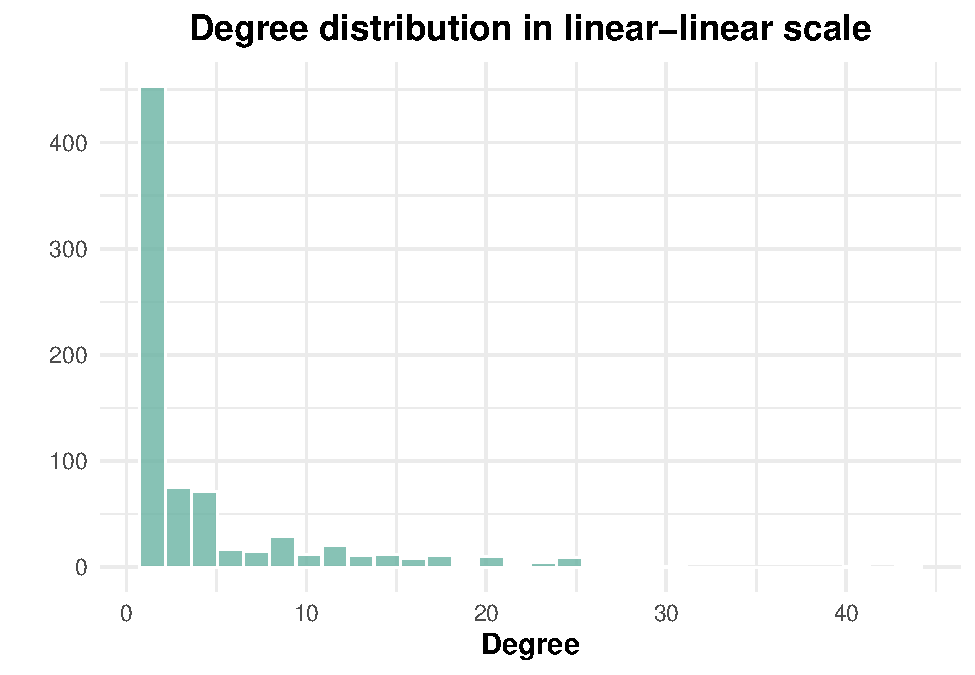
\includegraphics{export-network_files/figure-latex/unnamed-chunk-9-1.pdf}

\begin{Shaded}
\begin{Highlighting}[]
\CommentTok{\# In log{-}log scale}
\FunctionTok{ggplot}\NormalTok{() }\SpecialCharTok{+}
  \FunctionTok{geom\_histogram}\NormalTok{(}\FunctionTok{aes}\NormalTok{(}\AttributeTok{x =} \FunctionTok{degree}\NormalTok{(graph)),}
                 \AttributeTok{fill =} \StringTok{"\#69b3a2"}\NormalTok{, }\AttributeTok{color =} \StringTok{"white"}\NormalTok{, }\AttributeTok{alpha =} \FloatTok{0.8}\NormalTok{) }\SpecialCharTok{+}
  \FunctionTok{scale\_x\_log10}\NormalTok{() }\SpecialCharTok{+}
  \FunctionTok{scale\_y\_log10}\NormalTok{() }\SpecialCharTok{+}
  \FunctionTok{labs}\NormalTok{(}
    \AttributeTok{x =} \StringTok{"Degree (log scale)"}\NormalTok{,}
    \AttributeTok{y =} \StringTok{""}\NormalTok{,}
    \AttributeTok{title =} \StringTok{"Degree Distribution in Log{-}Log Scale"}
\NormalTok{  ) }\SpecialCharTok{+}
  \FunctionTok{theme\_minimal}\NormalTok{(}\AttributeTok{base\_size =} \DecValTok{14}\NormalTok{) }\SpecialCharTok{+}
  \FunctionTok{theme}\NormalTok{(}
    \AttributeTok{plot.title =} \FunctionTok{element\_text}\NormalTok{(}\AttributeTok{face =} \StringTok{"bold"}\NormalTok{, }\AttributeTok{hjust =} \FloatTok{0.5}\NormalTok{),}
    \AttributeTok{axis.title =} \FunctionTok{element\_text}\NormalTok{(}\AttributeTok{face =} \StringTok{"bold"}\NormalTok{)}
\NormalTok{  )}
\end{Highlighting}
\end{Shaded}

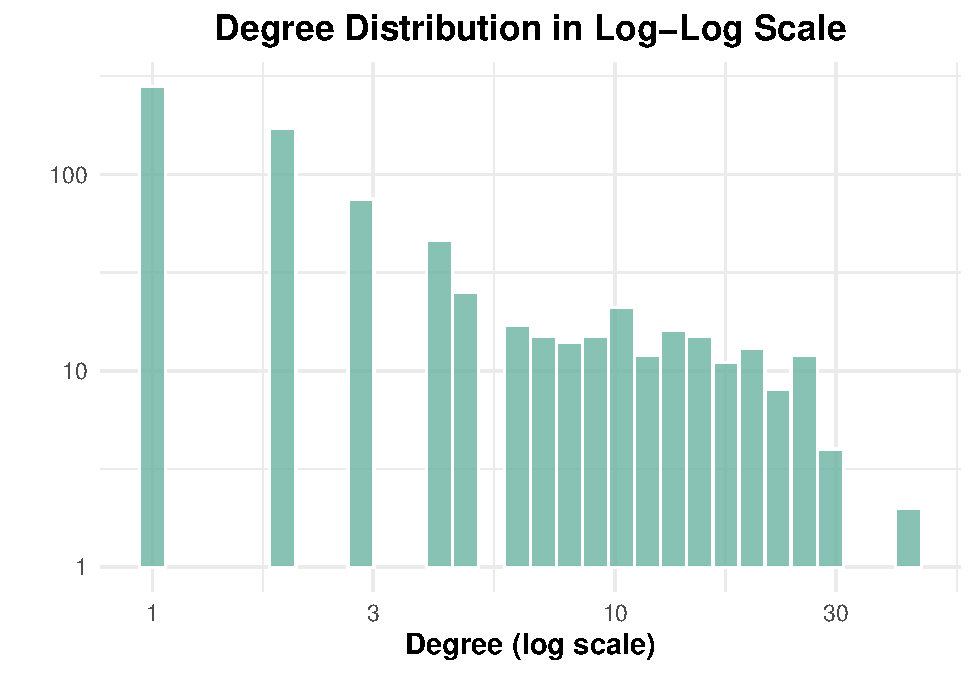
\includegraphics{export-network_files/figure-latex/unnamed-chunk-9-2.pdf}

We can observe that this network \textbf{does not exhibit typical
connectivity}: Its degree distribution is highly skewed and lacks a
clear peak. By being its degree distribution so broad there is not a
typical connectivity for a node. Most nodes have a very low degree,
while a few have very high degree. We observe a power-law-like
distribution, rather than a Poisson-like distribution, where most nodes
would have approximately the same number of links and no hubs. This is
what can usually be observed in social networks, but our product network
exhibits the same, indicating that some, but few products are exported
together with many different products by many countries, while the
majority of products are exported only by a few countries or by highly
specialized countries.

\begin{Shaded}
\begin{Highlighting}[]
\FunctionTok{max\_degree}\NormalTok{(graph)}
\end{Highlighting}
\end{Shaded}

\begin{verbatim}
## [1] 43
\end{verbatim}

The most connected node on our network has a degree of 43.

\begin{Shaded}
\begin{Highlighting}[]
\FunctionTok{which.max}\NormalTok{(}\FunctionTok{degree}\NormalTok{(graph))}
\end{Highlighting}
\end{Shaded}

\begin{verbatim}
## TRANSMISSION SHAFTS,CRANKS,BEARING HOUSINGS ETC. 
##                                              580
\end{verbatim}

The node with the highest degree is that of mechanical components,
indicating that there is no high specialization required to product
this. These are indeed products that are probably going to be used to
assemble more sophisticated goods and thus the demand for this product
is high everywhere and its supply chain is likely to be very globalized
with many countries producing them.

\subsection{4. What is the clustering coefficient (transitivity) in the
network?}\label{what-is-the-clustering-coefficient-transitivity-in-the-network}

\begin{Shaded}
\begin{Highlighting}[]
\FunctionTok{transitivity}\NormalTok{(graph, }\AttributeTok{type =} \StringTok{"global"}\NormalTok{)}
\end{Highlighting}
\end{Shaded}

\begin{verbatim}
## [1] 0.429691
\end{verbatim}

The global transitivity of this network is 0.4297, which is closer to 0
than to 1, indicating a modest tendency of clustering. Less than half of
the time, when two nodes share a common neighbor, they will also be
directly connected to each other. This could indicate that not always
countries tend to specialize on the same products.

\subsection{5. What is the assortativity (degree) in the
network?}\label{what-is-the-assortativity-degree-in-the-network}

\begin{Shaded}
\begin{Highlighting}[]
\FunctionTok{assortativity\_degree}\NormalTok{(graph)}
\end{Highlighting}
\end{Shaded}

\begin{verbatim}
## [1] 0.4571059
\end{verbatim}

The assortativity coefficient of this network is 0.4571 (greater than
0), indicating a moderate to strong tendency for nodes to connect with
others that have a similar degree. In other words, high-degree nodes
tend to connect with other high-degree nodes, and low-degree nodes tend
to connect with other low-degree nodes. This is a sign of assortative
mixing.

\subsection{6. Using the Louvain method, does the network have a
community structure? If so, what is its
modularity?}\label{using-the-louvain-method-does-the-network-have-a-community-structure-if-so-what-is-its-modularity}

\begin{Shaded}
\begin{Highlighting}[]
\NormalTok{louvain\_cluster }\OtherTok{\textless{}{-}} \FunctionTok{cluster\_louvain}\NormalTok{(graph, }\AttributeTok{weights =} \FunctionTok{E}\NormalTok{(graph)}\SpecialCharTok{$}\NormalTok{width)}

\FunctionTok{sizes}\NormalTok{(louvain\_cluster)}
\end{Highlighting}
\end{Shaded}

\begin{verbatim}
## Community sizes
##   1   2   3   4   5   6   7   8   9  10  11  12  13  14  15  16  17  18  19  20 
##  57 148  30  58 123  46  66  97  14   8  18   4  16   3   3  13  13   8   5   5 
##  21  22  23  24  25  26  27  28 
##   8   5   9   2   6   3   3   3
\end{verbatim}

\begin{Shaded}
\begin{Highlighting}[]
\FunctionTok{modularity}\NormalTok{(louvain\_cluster)}
\end{Highlighting}
\end{Shaded}

\begin{verbatim}
## [1] 0.7439031
\end{verbatim}

Yes, the network has a clear community structure. Using the Louvain
method, the network was partitioned into more than 20 communities. The
modularity value is \textbf{\textgreater0.7}, which is considered high
and indicates a strong modular (community) structure within the network.

We can also try to visualize these communities:

\begin{Shaded}
\begin{Highlighting}[]
\NormalTok{layout }\OtherTok{\textless{}{-}} \FunctionTok{layout\_with\_kk}\NormalTok{(graph)}

\CommentTok{\# Using igraph only}
\FunctionTok{plot}\NormalTok{(louvain\_cluster, graph,}
     \AttributeTok{layout =}\NormalTok{ layout,}
     \AttributeTok{vertex.size =} \FloatTok{0.1}\NormalTok{,}
     \AttributeTok{edge.width =} \FloatTok{0.1}\NormalTok{,}
     \AttributeTok{vertex.label =} \StringTok{""}\NormalTok{)}
\end{Highlighting}
\end{Shaded}

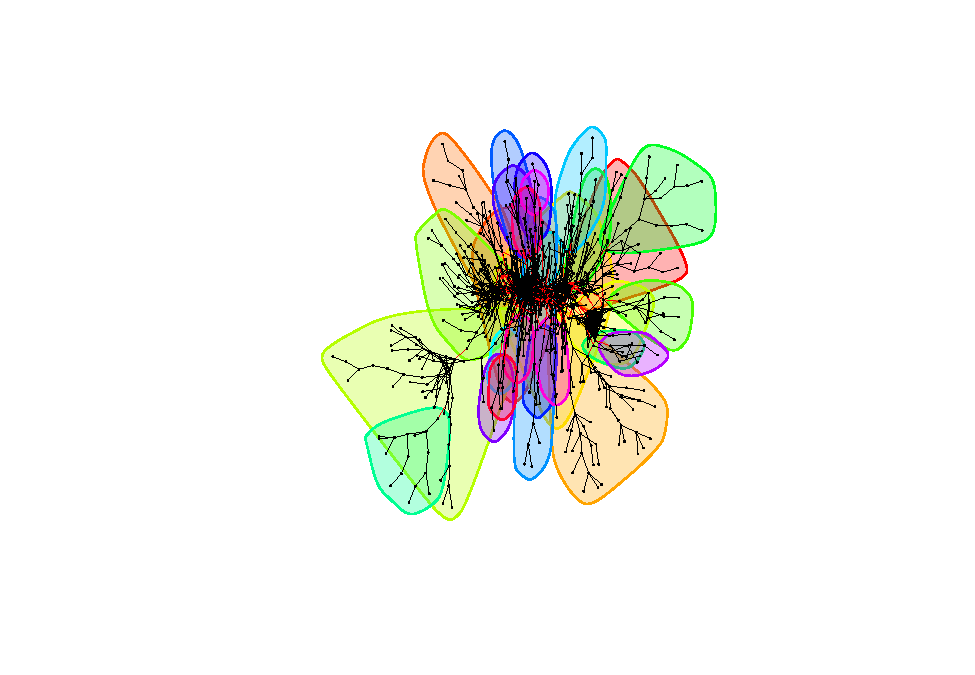
\includegraphics{export-network_files/figure-latex/unnamed-chunk-15-1.pdf}

\begin{Shaded}
\begin{Highlighting}[]
\CommentTok{\# Using ggraph}
\NormalTok{graph\_tbl }\OtherTok{\textless{}{-}} \FunctionTok{as\_tbl\_graph}\NormalTok{(graph)}
\FunctionTok{V}\NormalTok{(graph\_tbl)}\SpecialCharTok{$}\NormalTok{community }\OtherTok{\textless{}{-}} \FunctionTok{membership}\NormalTok{(louvain\_cluster)}
\FunctionTok{ggraph}\NormalTok{(graph\_tbl, }\AttributeTok{layout =} \StringTok{"kk"}\NormalTok{) }\SpecialCharTok{+}
  \FunctionTok{geom\_edge\_link}\NormalTok{(}\AttributeTok{width =} \FloatTok{0.1}\NormalTok{, }\AttributeTok{alpha =} \FloatTok{0.7}\NormalTok{, }\AttributeTok{color =} \StringTok{"grey"}\NormalTok{) }\SpecialCharTok{+}
  \FunctionTok{geom\_node\_point}\NormalTok{(}\FunctionTok{aes}\NormalTok{(}\AttributeTok{color =} \FunctionTok{as.factor}\NormalTok{(community)), }\AttributeTok{size =} \FloatTok{1.5}\NormalTok{) }\SpecialCharTok{+}
  \FunctionTok{theme\_void}\NormalTok{() }\SpecialCharTok{+}
  \FunctionTok{theme}\NormalTok{(}\AttributeTok{legend.position =} \StringTok{"none"}\NormalTok{)}
\end{Highlighting}
\end{Shaded}

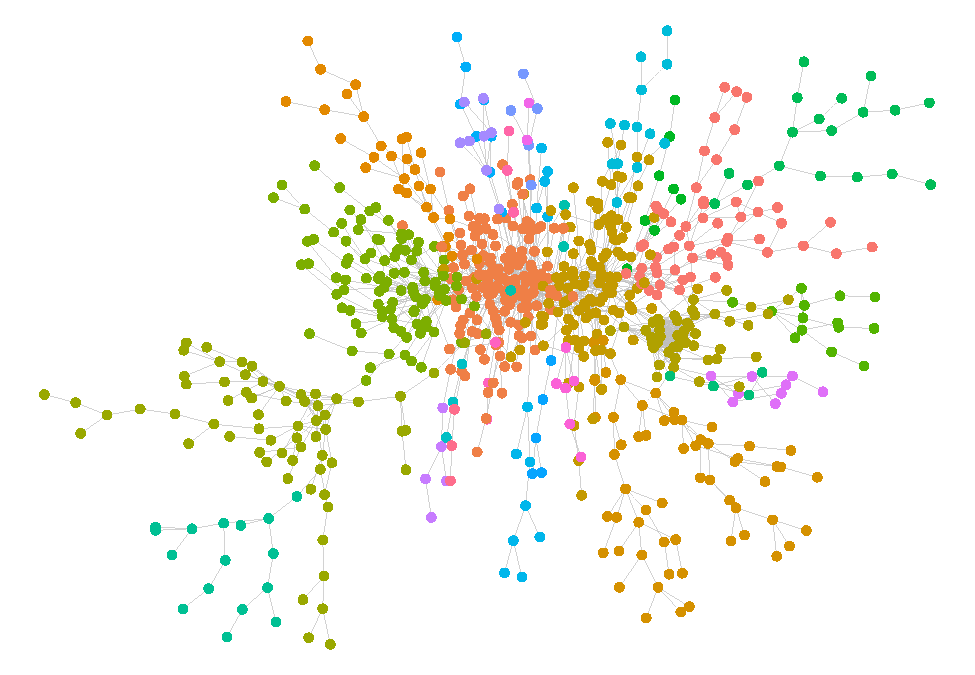
\includegraphics{export-network_files/figure-latex/unnamed-chunk-15-2.pdf}

\subsection{7. Test that the clustering coefficient in the network
cannot be statistically explain by a configuration model in which the
nodes have the same degree distribution as the
original.}\label{test-that-the-clustering-coefficient-in-the-network-cannot-be-statistically-explain-by-a-configuration-model-in-which-the-nodes-have-the-same-degree-distribution-as-the-original.}

\begin{Shaded}
\begin{Highlighting}[]
\NormalTok{original\_clustering }\OtherTok{\textless{}{-}} \FunctionTok{transitivity}\NormalTok{(graph, }\AttributeTok{type =} \StringTok{"global"}\NormalTok{)}
\end{Highlighting}
\end{Shaded}

Create 1000 random configuration models and register the clustering
coefficient for each one of this generated model.

\begin{Shaded}
\begin{Highlighting}[]
\NormalTok{num\_simulations }\OtherTok{\textless{}{-}} \DecValTok{1000}
\CommentTok{\# Initializing a vector}
\NormalTok{simulated\_clustering }\OtherTok{\textless{}{-}} \FunctionTok{numeric}\NormalTok{(num\_simulations)}
\CommentTok{\# Simulating the graphs and saving their transitivity}
\ControlFlowTok{for}\NormalTok{ (i }\ControlFlowTok{in} \DecValTok{1}\SpecialCharTok{:}\NormalTok{num\_simulations) \{}
\NormalTok{  config\_graph }\OtherTok{\textless{}{-}} \FunctionTok{sample\_degseq}\NormalTok{(}\FunctionTok{degree}\NormalTok{(graph), }\AttributeTok{method =} \StringTok{"vl"}\NormalTok{)  }
\NormalTok{  simulated\_clustering[i] }\OtherTok{\textless{}{-}} \FunctionTok{transitivity}\NormalTok{(config\_graph, }\AttributeTok{type =} \StringTok{"global"}\NormalTok{)}
\NormalTok{\}}
\end{Highlighting}
\end{Shaded}

Here we use the method ``vl'' (Viger--Latapy) as it is the one suggested
for undirected connected graphs.

Once we have generated the networks we want to proceed with evaluation
and test of statistical difference.

\begin{Shaded}
\begin{Highlighting}[]
\NormalTok{original\_clustering}
\end{Highlighting}
\end{Shaded}

\begin{verbatim}
## [1] 0.429691
\end{verbatim}

\begin{Shaded}
\begin{Highlighting}[]
\FunctionTok{mean}\NormalTok{(simulated\_clustering)}
\end{Highlighting}
\end{Shaded}

\begin{verbatim}
## [1] 0.03402928
\end{verbatim}

\begin{Shaded}
\begin{Highlighting}[]
\FunctionTok{t.test}\NormalTok{(}\AttributeTok{x =}\NormalTok{ simulated\_clustering, }\AttributeTok{mu =}\NormalTok{ original\_clustering, }\AttributeTok{alternative =} \StringTok{"two.sided"}\NormalTok{)}
\end{Highlighting}
\end{Shaded}

\begin{verbatim}
## 
##  One Sample t-test
## 
## data:  simulated_clustering
## t = -4845.7, df = 999, p-value < 2.2e-16
## alternative hypothesis: true mean is not equal to 0.429691
## 95 percent confidence interval:
##  0.03386905 0.03418951
## sample estimates:
##  mean of x 
## 0.03402928
\end{verbatim}

We tested whether the clustering coefficient of the original network can
be explained solely by its degree distribution, by comparing it to 1000
configuration model networks with the same degree sequence. The original
network's clustering coefficient was \textbf{0.4297}, while the average
clustering coefficient from the configuration models was \textbf{0.034}.

Therefore we can conclude that the clustering structure in the original
network \textbf{cannot be explained} by degree distribution alone --- it
has significant non-random structure peculiar to the network.

\subsection{8. Visualize the neighborhood of the node with the largest
centrality
(closeness)}\label{visualize-the-neighborhood-of-the-node-with-the-largest-centrality-closeness}

\begin{Shaded}
\begin{Highlighting}[]
\FunctionTok{which.max}\NormalTok{(}\FunctionTok{closeness}\NormalTok{(graph))}
\end{Highlighting}
\end{Shaded}

\begin{verbatim}
## SLAG WOOL.ROCK WOOL AND SIMILAR MINERAL WOOLS 
##                                           453
\end{verbatim}

We discovered that the node with the largest centrality/closeness is
``SLAG WOOL.ROCK WOOL AND SIMILAR MINERAL WOOLS''. Apparently these are
insulating materials coming from minerals.

\begin{Shaded}
\begin{Highlighting}[]
\FunctionTok{head}\NormalTok{(}\FunctionTok{neighbors}\NormalTok{(graph,}\StringTok{"SLAG WOOL.ROCK WOOL AND SIMILAR MINERAL WOOLS"}\NormalTok{))}
\end{Highlighting}
\end{Shaded}

\begin{verbatim}
## + 6/774 vertices, named, from 0ef3264:
## [1] TRAILERS & SPECIALLY DESIGNED CONTAINERS          
## [2] PARTS OF THE MACHINERY OF 723.41 TO 723.46        
## [3] MATERIALS OF RUBBER(E.G.,PASTES.PLATES,SHEETS,ETC)
## [4] OTHER VEHICLES,NOT MECHANICALLY PROPELLED,PARTS   
## [5] PARTS OF THE MACHINERY OF 744.2-                  
## [6] MISCELLANEOUS ART.OF MATERIALS OF DIV.58
\end{verbatim}

These are some of the neighbors of our node of interest.

We'll now plot its neighbors.

\begin{Shaded}
\begin{Highlighting}[]
\NormalTok{neigh\_graph }\OtherTok{\textless{}{-}} \FunctionTok{make\_neighborhood\_graph}\NormalTok{(graph,}
                                       \AttributeTok{order =} \DecValTok{1}\NormalTok{, }
                                       \StringTok{"SLAG WOOL.ROCK WOOL AND SIMILAR MINERAL WOOLS"}\NormalTok{)[[}\DecValTok{1}\NormalTok{]]}

\NormalTok{g }\OtherTok{\textless{}{-}} \FunctionTok{as\_tbl\_graph}\NormalTok{(neigh\_graph)}

\FunctionTok{ggraph}\NormalTok{(g, }\AttributeTok{layout =} \StringTok{\textquotesingle{}fr\textquotesingle{}}\NormalTok{) }\SpecialCharTok{+}
  \FunctionTok{geom\_edge\_link}\NormalTok{(}\AttributeTok{alpha =} \FloatTok{0.5}\NormalTok{, }\AttributeTok{width =} \DecValTok{1}\NormalTok{) }\SpecialCharTok{+}
  \CommentTok{\# Colouring of a different colour our central node}
  \FunctionTok{geom\_node\_point}\NormalTok{(}\AttributeTok{size =} \DecValTok{5}\NormalTok{, }
                  \FunctionTok{aes}\NormalTok{(}\AttributeTok{color =}\NormalTok{ name }\SpecialCharTok{==} \StringTok{"SLAG WOOL.ROCK WOOL AND SIMILAR MINERAL WOOLS"}\NormalTok{)) }\SpecialCharTok{+}
  \FunctionTok{geom\_node\_text}\NormalTok{(}\FunctionTok{aes}\NormalTok{(}\AttributeTok{label =}\NormalTok{ name), }
                 \AttributeTok{repel =} \ConstantTok{TRUE}\NormalTok{, }
                 \AttributeTok{size =} \DecValTok{3}\NormalTok{, }
                 \AttributeTok{color =} \StringTok{"steelblue"}\NormalTok{, }
                 \AttributeTok{check\_overlap =} \ConstantTok{TRUE}\NormalTok{) }\SpecialCharTok{+}
  \FunctionTok{guides}\NormalTok{(}\AttributeTok{color =} \StringTok{"none"}\NormalTok{) }\SpecialCharTok{+}    
  \FunctionTok{theme\_void}\NormalTok{()}\SpecialCharTok{+}
  \FunctionTok{labs}\NormalTok{(}\AttributeTok{title =} \StringTok{"Neighborhood of Node with Highest Closeness Centrality"}\NormalTok{)}
\end{Highlighting}
\end{Shaded}

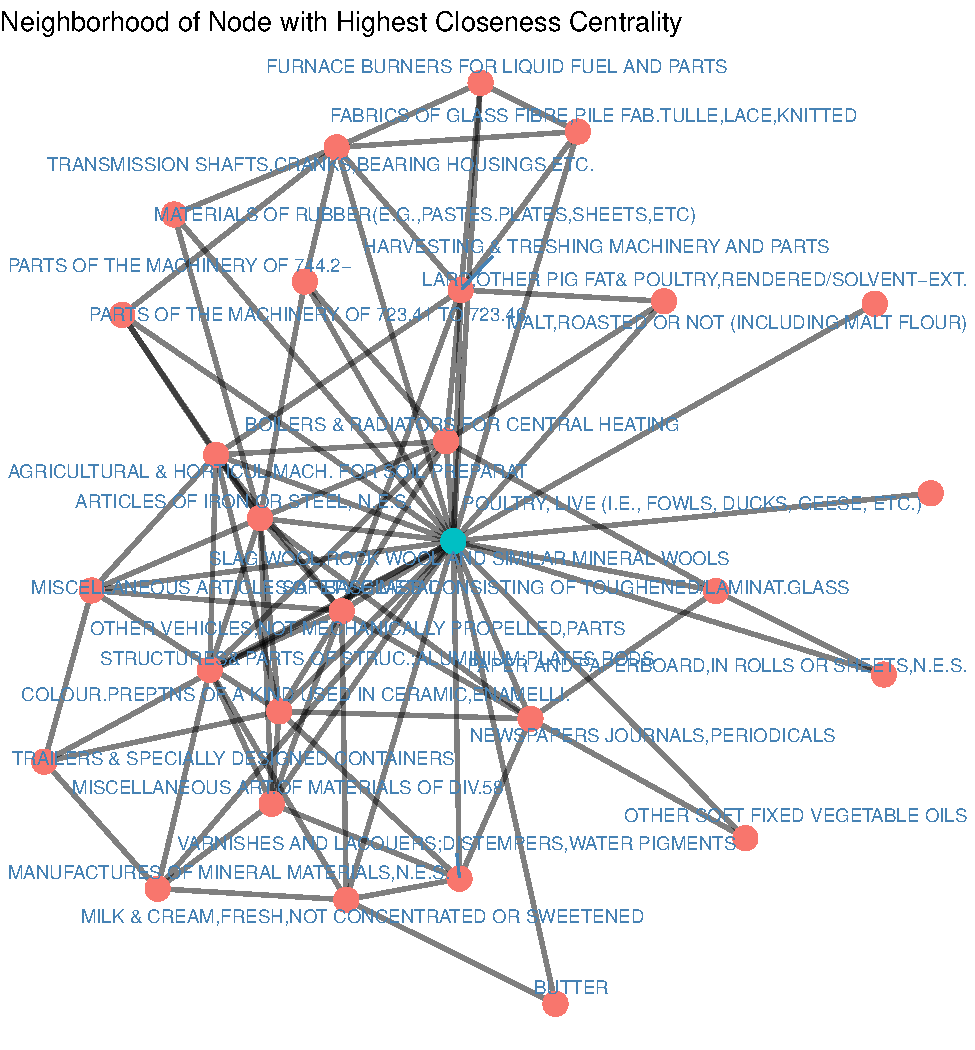
\includegraphics{export-network_files/figure-latex/unnamed-chunk-22-1.pdf}

This plot looks a little bit messy, as the labels are quite long and
difficult to read. However, if we hide all the labels, we lose a lot of
valuable information. Therefore, we decided to use the visNetwork
package to create an interactive graph, which allows us to freely drag
nodes around and better explore the names of each node:

\begin{Shaded}
\begin{Highlighting}[]
\FunctionTok{library}\NormalTok{(visNetwork)}
\NormalTok{nodes }\OtherTok{\textless{}{-}} \FunctionTok{data.frame}\NormalTok{(}\AttributeTok{id =} \FunctionTok{V}\NormalTok{(g)}\SpecialCharTok{$}\NormalTok{name, }\AttributeTok{label =} \FunctionTok{V}\NormalTok{(g)}\SpecialCharTok{$}\NormalTok{name)}
\NormalTok{edges }\OtherTok{\textless{}{-}} \FunctionTok{data.frame}\NormalTok{(}\AttributeTok{from =} \FunctionTok{as.character}\NormalTok{(}\FunctionTok{ends}\NormalTok{(g, }\FunctionTok{E}\NormalTok{(g))[,}\DecValTok{1}\NormalTok{]), }\AttributeTok{to =} \FunctionTok{as.character}\NormalTok{(}\FunctionTok{ends}\NormalTok{(g, }\FunctionTok{E}\NormalTok{(g))[,}\DecValTok{2}\NormalTok{]))}

\FunctionTok{visNetwork}\NormalTok{(nodes, edges) }\SpecialCharTok{\%\textgreater{}\%}
  \FunctionTok{visEdges}\NormalTok{(}\AttributeTok{color =} \FunctionTok{list}\NormalTok{(}\AttributeTok{color =} \StringTok{"gray"}\NormalTok{, }\AttributeTok{hover =} \StringTok{"red"}\NormalTok{)) }\SpecialCharTok{\%\textgreater{}\%}
  \FunctionTok{visNodes}\NormalTok{(}\AttributeTok{size =} \DecValTok{15}\NormalTok{, }\AttributeTok{color =} \FunctionTok{list}\NormalTok{(}\AttributeTok{background =} \StringTok{"lightblue"}\NormalTok{, }\AttributeTok{border =} \StringTok{"darkblue"}\NormalTok{)) }\SpecialCharTok{\%\textgreater{}\%}
  \FunctionTok{visOptions}\NormalTok{(}\AttributeTok{highlightNearest =} \ConstantTok{TRUE}\NormalTok{, }\AttributeTok{nodesIdSelection =} \ConstantTok{TRUE}\NormalTok{) }\SpecialCharTok{\%\textgreater{}\%}
  \FunctionTok{visLayout}\NormalTok{(}\AttributeTok{randomSeed =} \DecValTok{123}\NormalTok{)}
\end{Highlighting}
\end{Shaded}

\begin{verbatim}
## file:////private/var/folders/5k/zh67w_yx2fj10t7z34l2ct7m0000gn/T/RtmpzAAnHd/file13427a1bc9d6/widget134236603f3b.html screenshot completed
\end{verbatim}

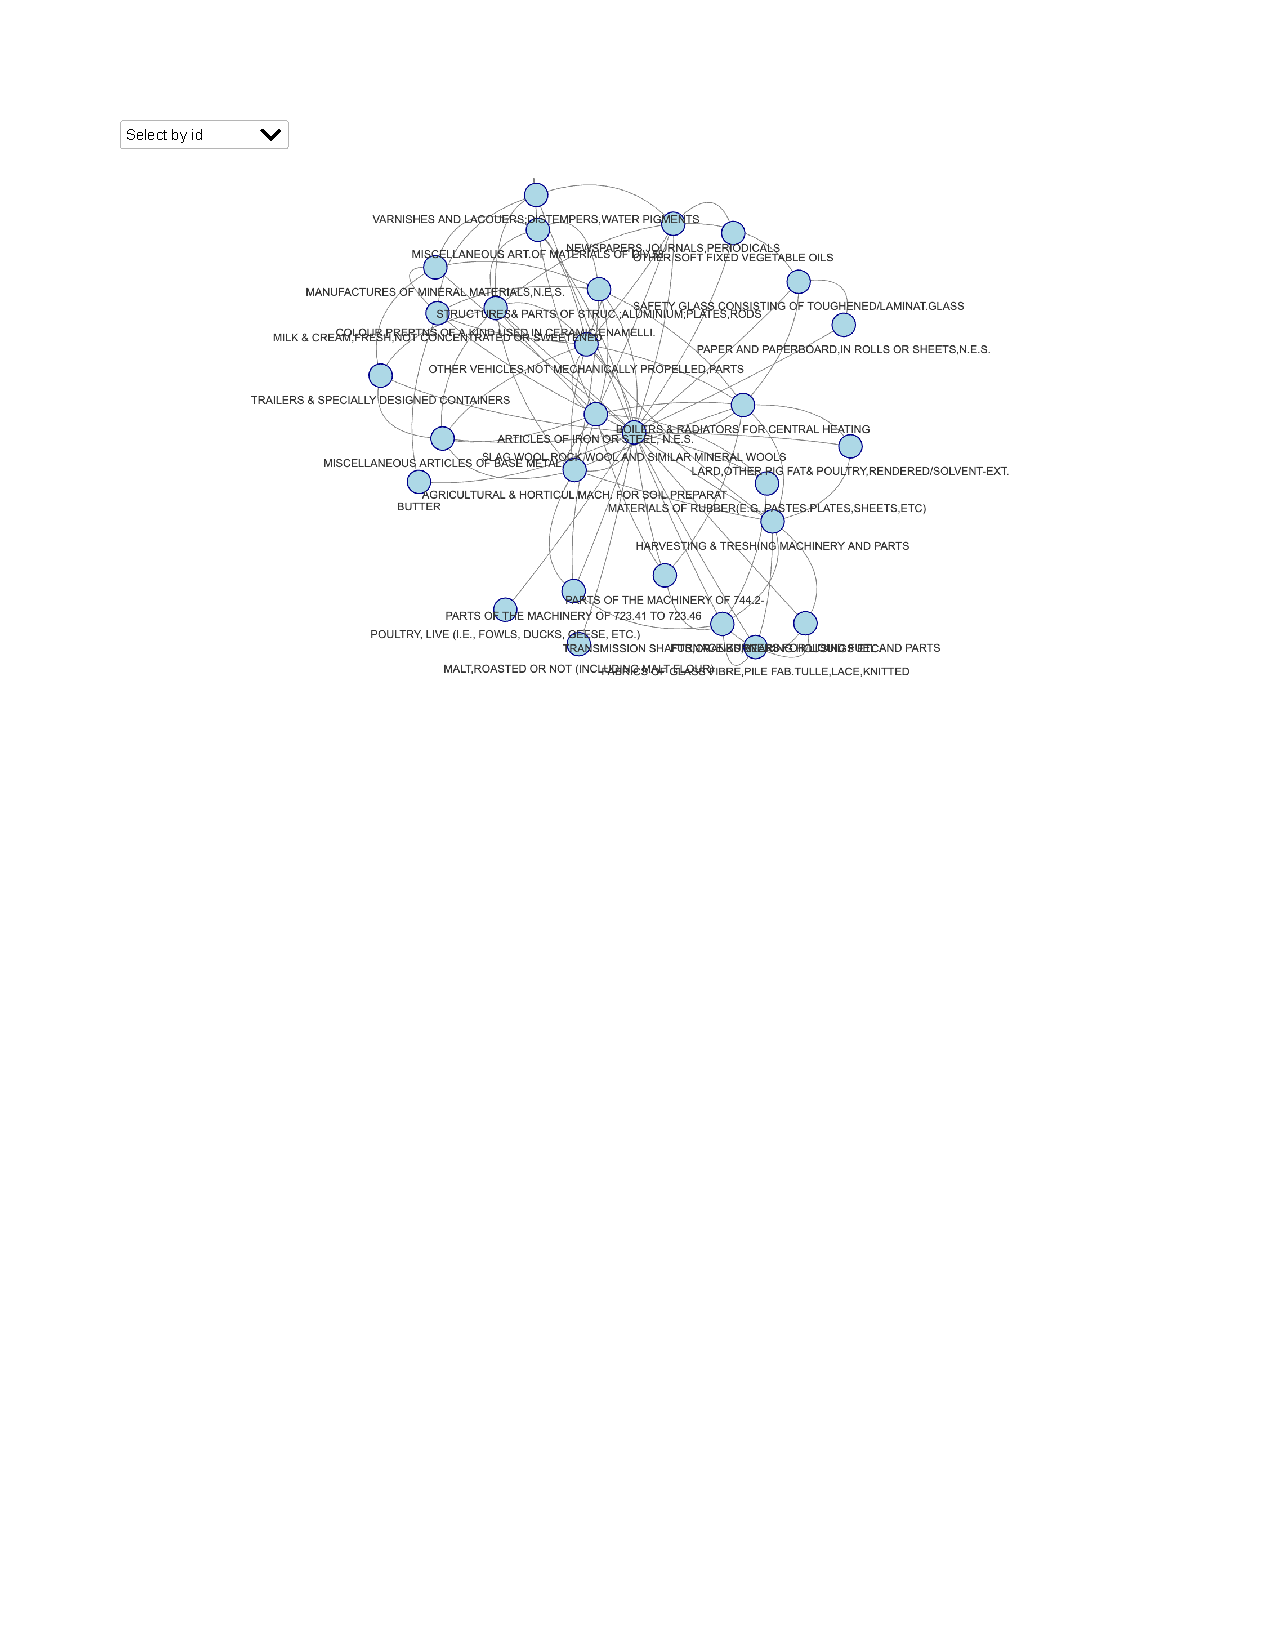
\includegraphics{export-network_files/figure-latex/unnamed-chunk-23-1.pdf}

NOTE: As these is a \texttt{.pdf} document we are only able to show a
screeenshot of the graph

\end{document}
